\chapter{Model realization\label{chap:modelReal}}


%Detailed enough to be able to reproduce
%Pseudocode where applicable
%Explain along figure?
%Include technology that's used
%How did we realize/achieve the ideas?
%Present what kind of assumptions/prior knowledge is made!!

\begin{itemize}
	\item Actual architectures resemble concepts closely
	\item Crux lies in the regression model (AITM)
\end{itemize}

In order to evaluate the developed ideas, prototypes of the two concepts described in the previous section have been implemented in Python. Both prototypes are developed as such that they can be evaluated in the same way in the next chapter. The implementations try to follow the presented concepts very closely. As such the general data flow is the same as was presented in the figures  \ref{fig:PairPrediction}, \ref{fig:GatePrediction} and \ref{fig:GatePlanning}.
Relevant decisions and assumptions made specifically for the implementation are highlighted and explained in this chapter. %TODO maybe needs to be changed

Section \ref{sec:basics} starts with describing common design decisions made that apply to both concepts. Afterwards the relevant implementations details regarding the two prototypes are presented in section \ref{sec:pairRealization} for the interaction state concept and in section \ref{sec:gateRealization} for the object state concept. Finally, section \ref{sec:technologies} describes the used technologies such as the underlying regression and classification model and the implementation of the inverse model in detail.

\section{Basics \label{sec:basics}}

%The following descriptions and assumptions are accurate for all realizations independent of the underlying concept.

\begin{itemize}
\item Action primitives
\item 
\end{itemize}

%\subsection{Single timestep}
%TODO consider if this makes sense/is required
%One way to learn pushing interactions is to learn the trajectories of entire interactions. While this is possible, for example with a Hidden Markov Model \cite{hmm} and has been done successfully by [TODO look up name] \cite{hmmTrajectory}, it requires labeled training data. %TODO
%More precisely, it requires the models to know when a trajectory starts and when it finishes. Since the model presented here are supposed to learn incrementally by self exploration or at least in an online manner without being provided labeled data from the outside, the models would need to derive the start and endpoints of an interaction automatically. 
%
%The models presented here do not predict entire interactions but rather make small predictions at each timestep in order to avoid the need for such segmentation. This also means that these models are coupled closely to their environment and get updates at each timestep. The actual duration between two updates is not predetermined or restricted by the models presented here. The longer the duration between updates, the more the object states change during an interaction. 
%TODO maybe rearrange the sentences

\subsection{Available information about objects}

The kind of information that is provided by the environment obviously depends on the sensors that are available to the robot. From the information provided by these sensors, features can be computed. The models themselves are greatly independent on what features are actually used. In fact the models do not require any knowledge about what the features represent for prediction and none is provided. This allows the exact same model to be used in various settings with different features, for example if additional or different sensors are available. In order to yield good results, the used features obviously need to have the necessary expressiveness.

Unfortunately, the model does need to have some partial knowledge about the features when it comes to planning as will be further explained in the corresponding sections of both models.

These prototypes were evaluated using a physics simulation, further explained in section \ref{sec:simulation}. From this simulation the information in table \ref{tab:availInformation} is provided for each object at each update.

\begin{table}[h!]
	\centering
	\begin{tabular*}{\textwidth}{@{\extracolsep{\fill} } l l}
		\textbf{Feature} & \textbf{Description} \\ 
		\hline \hline 
		x Position & Global x position of the object \\
		y Position & Global y position of the object \\
		Orientation & Global orientation around the z-axis of the object \\
		x Velocity & Global x velocity of the object \\
		y Velocity & Global y velocity of the object \\
		\hline 
	\end{tabular*} 
	\caption{Summary of all information about objects that is available at each update step from the environment in the given setting.}
	\label{tab:availInformation}
\end{table}

Furthermore,  a unique identifier, the shape and size of the objects are known and can be used to compute additional features for the model. What kind of features are computed from this information is a design decision of the user of these models. Because of the dependence on the used metric in the underlying regression model, using more features might worsen the performance of the models. 



\subsection{Action primitives}
In the scope of this thesis, the action primitives allow to set the two dimensional velocity of the actuator. Although, velocities are set, the models assume that an action is selected and performed at every iteration. In general, the nature of the action is not all that important to the models as long as it can be represented as a vector. In this case a two dimensional vector is used representing the x- and y-velocity respectively. The velocities are given according to the global coordinate system of robot. 

\subsection{Used regression and classification model}

As already stated in the introduction and motivated in chapter \ref{chap:stateOfTheArt}, this thesis uses a memory based approach to learn the interactions. For this end, a special adaptation of the \gls{gng} has been developed which can be used for regression as well as classification tasks. This \gls{aitm}, explained in section \ref{sec:ITM}, is used for all regression and classification models used in both prototypes unless otherwise mentioned. 

\subsection{Using local features and predicting differences}
%TODO rewrite
\begin{itemize}
\item Local features make the assumption that everything behaves the same regardless of the configuration
\item Difference prediction needs to be used when using local features
\item Difference prediction is also possible with global features and without the assumption
\item Difference prediction reduces output space, not sure if I want to write about this
\end{itemize}
Both prototypes only use local features as inputs for their trained regression and classification models as can be seen in sections \ref{sec:intFeatures} and \ref {sec:gateFeatures}.
This means that in the interaction states as well as the Relative Interaction Features of the object state model represent all features relative to some reference object's coordinate frame. The great advantage of this approach is that the interactions can be learned regardless of the object's actual configuration in the environment. %TODO


Both concepts describe that the local models predict the next state of the interaction and object states respectively. In the realization presented here, only the changes in the states are predicted instead of the actual resulting states. 

Using only differences greatly reduces the complexity of the problem. Instead of learning the interaction behavior of objects at every configuration in the environment separately, it is sufficient to learn the behavior independent of the configuration. In fact training data from all different configurations can be used to learn about the same interaction. Consequently, generalization about different configurations in the environment come for free. 

%TODO consider if the following is even true. Can't predicting differences even be used with environment effects?
Learning on the differences makes the assumption that similar interactions behave in the same way regardless of the actual configuration. Considering the given situation this assumes that an object will always move in the same way no matter where and how it is located in the environment. In other words, the effects of an interaction are only dependent on the relation between the objects involved and not on their global attributes. For the given task of pushing interactions this assumption will hold true as long as the environment only has a constant effect on the objects. The environment used for the evaluations, described in section \ref{sec:environment}, fulfills these conditions since it only affects the objects through gravity and friction, which are constant throughout the entire environment. 

In more realistic environments, where this assumption does not hold true, the differences can still be used. However, in this case, the used input features need to contain the information about the influence of the environment or the current object configuration. 



\section{Modeling pairwise interaction \label{sec:pairRealization}}

%\begin{itemize}
%	\item feature selection? (currently not implemented in latest version)
%\end{itemize}

The implementation of the pairwise interaction model also contains the components visualized in figure \ref{fig:PairOverview}. From these components, three different parts are trained:
The Abstract Collection Selector trains a classifier that selects any of the $n$ learned Abstract Collections. Within each Abstract Collections, there exist a local forward model which performs the predictions. Additionally, the Abstract Collections contain an inverse model, which return preconditions that result in a specific change of the interaction state. The forward model as well as the selector both use the same underlying mechanism with the \gls{aitm}. For the reasons explained in section \ref{sec:invModel}, the special inverse model is used.

Algorithm \ref{alg:intUpdate} explains the steps that are performed each time new information is received from the environment.

\begin{algorithm}
	\KwIn{New worldstate ws}
	\KwIn{Used action a}
	\KwData{Last worldstate ws$_\text{old}$}
	\KwData{Set of Abstract Collections L}
	\KwData{Abstract Collection Selector ACS}
	\BlankLine
	\ForEach{interaction state i $\in$ ws}{
		newEpisode = Episode(i$_\text{old}$, a, i) \\
		S = newEpisode.changedFeatures() \\
		\tcc*[h]{Check if a corresponding AC already known} \\
		\If{S $\notin$ L}{
			newAC = AbstractCollection(S) \\
			L = L $\cup$ newAC 
		}
		AC = L$_\text{S}$ \tcc*[f]{The Abstract Collection responsible for S} \\
		update AC with newEpisode \\
		update ACS with i$_\text{old}$, a and AC
	}
	\caption{Prediction of the update steps in the pairwise interaction model.}
	\label{alg:intUpdate}
\end{algorithm}

The changed feature set S is basically computed according to equation \ref{eq:difSet}. However, it is important to note, that the $Post$ state needs to be transformed to the same coordinate frame as the $Pre$ state before computing the differences. The exact computation is shown in section \ref{sec:episodes} where the structure of these episodes is explained.

When updating an Abstract Collection both its forward and inverse model need to be updated. The forward model as well as the inverse model are trained using the combination of the old interaction state i$_\text{old}$ and the action primitive a as input and the difference vector d between the old interaction state and the new one as desired output. The exact training of the \gls{aitm} is explained in section \ref{sec:ITM} while the training of the inverse model is explained in section \ref{sec:invModelRealization}.

The Abstract Collection Selector is trained on the same combination of i$_\text{old}$ and a as input, but it uses the identifier of the responsible Abstract Collection as desired output.
Since the selector also uses the \gls{aitm} as classifier, the exact update rules are explained below.

When used for the prediction the model follows the process visualized in figure \ref{fig:PairPrediction} and described in section \ref{sec:pairPrediction}. The only difference is that, only changes are predicted by the local forward models. Learning on the differences instead of the actual results, allows to abstract from the actual scenario. That way all pushing interactions that result in a similar orientation can be treated the same


%The model itself only works on interaction states and action primitives. The specific structure and content of these features is explained in section \ref{sec:intFeatures}.


\subsection{Used features \label{sec:intFeatures}}

The pairwise interaction model basically only uses the interaction state and the action primitive vector as feature vectors. The actual composition of the interaction state depends on the objects that need to be represented. For this thesis, only simple objects are present in the scene which allows fairly simple interaction states as described in table \ref{tab:pairInteractionFeatures}.

\begin{table}
	\centering
	\begin{tabular*}{\textwidth}{@{\extracolsep{\fill} } l l}
		\textbf{Feature} & \textbf{Description} \\ 
		\hline \hline 
		 Id 1 & Identifier of the reference object \\ 
		 Id 2 & Identifier of the second object \\ 
		 Local x Position & Local x position of the reference object \\
		 Local y Position & Local y position of the reference object \\
		 Local Orientation & Local orientation of the reference object \\
		 Relative x Position & Relative x position of the second object \\
		 Relative y Position & Relative y position of the second object \\
		 Relative Orientation & Relative orientation of the second object \\
		\hline 
	\end{tabular*} 
	\caption{This table shows exemplary features used to represent one interaction state. Relative positions and velocities refer to the coordinate system of the reference object.}
	\label{tab:pairInteractionFeatures}
\end{table}

Furthermore, the interaction state contains the information required for the transformations. Specifically, the matrix $T$ to transform from the local coordinate frame back to the global 
frame, its inverse $T^{-1}$ and the orientation of the reference object in the global coordinate frame.

The model assumes, that these interaction states come directly from the environment. Transformations from and to the actual object states need to be performed outside of the actual model. This is achieved by introducing a \textit{Worldstate}. From the point of view of the model, this world state is simply a collection of all interaction states in the environment. At each update from the environment, a new Worldstate is computed from the information provided. The model predicts a new Worldstate by making predictions about all interaction states that are included in a given Worldstate. Since one is usually more interested in the actual object states, the model finalizes the Worldstate after all interaction states have been predicted. This finalization extracts the object state predictions from the predicted interaction states. 

The interaction states are computed as follows:
In this case all features are computed by transforming the global features of both objects given by the environment to the local coordinate frame. Consider two objects $o_1$ and $o_2$ with positions $\vec{p}_1$ and $\vec{p}_2$ and orientations $\alpha_1$ and $\alpha_2$ respectively. First the transformation matrices $T$ and $T^{-1}$ are computed from the reference object's position and orientation:

\begin{equation}
T = \begin{pmatrix}
\cos(\alpha_1) & -\sin(\alpha_1) & px_1 \\
\sin(\alpha_) & \cos(\alpha_1) & py_1 \\
0.0 & 0.0 & 1.0
\end{pmatrix}
\qquad
T^{-1} = inv(T)
\end{equation}

$px_1$, $py_1$ correspond to the $x$ and $y$ dimensions of the position $\vec{p}_1$. With the help of the transformation matrix $T^{-1}$ it is possible to compute the local positions, e.g.:

\begin{equation}
\vec{p}' = T^{-1} \times \vec{p_1}^*
\end{equation}

where $\vec{p}_1^*$ is the homogeneous vector of $\vec{p}_1$. Since $\vec{p}'$ is also in homogeneous coordinates, only the first two components are used for the interaction state. The local and relative orientations are computed by subtracting the orientation of the reference object from the given orientations. In fact by doing this, all local fields in the interaction state will be zero after the computation. However, these fields are still required. The Abstract Collections predict the change in the current interaction state. In order to extract the predicted object states from the interaction state, changes in the reference object need to be predicted as well. 

The object states are extracted by using the inverse transformation. Since the structure of the interaction states are known outside of the model, the predicted local position $\vec{q}$ can easily be extracted. Using the homogeneous coordinates $\vec{q}^*$ of $\vec{q}$, the prediction for the actual object's position $\vec{p}_{pred}$ can be computed:

\begin{equation}
\vec{p}_{pred}^* = T \times \vec{q}^*
\end{equation}

Velocities can be computed analog if needed.
In order to get the global orientation, the reference object's orientation simply needs to be added to the predicted orientation. 

\subsection{Episodes \label{sec:episodes}}

\begin{itemize}
\item Explain difference computation
\end{itemize}










\section{Object space with gating function \label{sec:gateRealization}}

The realization consists mainly of the parts that are visualized in figure \ref{fig:GateOverview}. 

Algorithm \ref{alg:gatePrediction} shows how a prediction for one object is performed. 


\begin{algorithm}
	\KwIn{Predicted actuator state from action primitive, object state}
	\KwOut{Predicted object state}
	\BlankLine
	relFeature = computeRelativeFeatures(objectState, actuatorState)\\
	\eIf{Gate(relFeatures)}{
		predictedChange = getPrediction(relFeatures) \\
		return add(objectState, predictedChange)
		}{
		return objectState
		}	
	\caption{Prediction pseudocode}
	\label{alg:gatePrediction}
\end{algorithm}

The pseudo function \textit{getPrediction} first selects the responsible forward model before the change is predicted. This selection is being performed based on the identifier of the reference object. If no local model has been trained for the reference object, the predictor tries to find a forward model that is responsible for similar objects. If no suitable forward model can be found, a zero change prediction is returned. This means that the object state remains unchanged.


\subsection{Used features \label{sec:gateFeatures}}

This model uses different kind of feature representations. The object states consist of their object specific features. The once that are most important are dynamic features, meaning the features that can actually change. These features are summarized in table \ref{tab:gateObjectFeatures}.

\begin{table}
	\centering
	\begin{tabular}{|c|c|}
		\hline Feature & Description \\ 
		\hline x Position & Global x position in the environment \\ 
		\hline y Position & Global y position in the environment \\ 
		\hline Orientation & Object rotation around the z-axis of the global coordinate system \\ 
		\hline 
	\end{tabular} 
	\caption{Table showing the different dynamic features used to represent objects.}
	\label{tab:gateObjectFeatures}
\end{table}

On top of these dynamic features, static onces like an identifier or information about the shape of the object is included. For example, in order to compute some of the relative interaction features the width and height of the objects are required. Furthermore, the model stores not only the current state of each object but also the previous one. This is required in order to make finite difference estimations about the objects dynamics such as velocity. 
The relative interaction features are summarized in table \ref{tab:gateInteractionFeatures}. 

\begin{table}
	\centering
	\begin{tabular}{|c|c|}
		\hline Feature & Description \\ 
		\hline Id 1 & Identifier of the reference object \\ 
		\hline Id 2 & Identifier of the second object \\ 
		\hline Distance & Closest distance between the two objects \\
		\hline Closing & Describes how much the objects are moving towards each other \\
		\hline Relative x Position & Relative x position of the second object \\
		\hline Relative y Position & Relative y position of the second object \\
		\hline Relative x Velocity & Relative x velocity of the second object \\
		\hline Relative y Velocity & Relative y velocity of the second object \\
		\hline 
	\end{tabular} 
	\caption{Table summarizing the different relative interaction features used to make predictions about interactions. Relative positions and velocities refer to the coordinate system of the reference object.}
	\label{tab:gateInteractionFeatures}
\end{table}

The \textit{Closing} feature $c$ is computed as described in equation \ref{eq:closing} and visualized in figure \ref{fig:closing}.

\begin{equation}
  c = \vec{n} \cdot \vec{rv}
 \label{eq:closing}
\end{equation}

where $\vec{n}$ represents the normal from the reference object towards the second object and $\vec{rv}$ represents the non normalized relative velocity vector of that second object. This equates to the cosine between these two vectors weighted by the magnitude of the relative velocity. This feature is minimal when the second object is moving directly towards the reference object. A positive closing value on the other hand indicates that the objects are moving away from each other. When the feature becomes 0 it indicates that the distance will not change. As mentioned above, the relative velocity is estimated by the finite difference of the current and last position.

The other relative features are computed by transforming their global counterparts to the coordinate system of the reference object. Equation \ref{eq:trans} shows this exemplary for the position:

\begin{equation}
	\vec{relPos} = M \times \vec{gPos}
\label{eq:trans}
\end{equation}

where $M$ is the three dimensional transformation matrix computed from the reference objects orientation and global position. $\vec{gPos}$ is the position vector of the second object extended by a $1$ in order to allow translation along the rotation. 

\begin{figure}
	\centering
	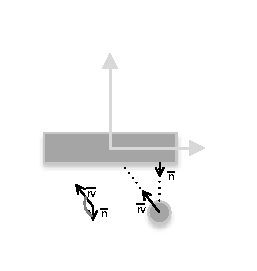
\includegraphics[scale = 1.5]{closing.pdf}
	\caption{Visualization of the closing feature. The gray half circle shows the angle whose cosine is basically computed for the feature.} 
	\label{fig:closing}
\end{figure}

\subsection{Gate}

The gate trains a binary classifier on the relative interaction features about if an interaction takes place or not. 



\section{Used technologies \label{sec:technologies}}

\subsection{Inverse Model \label{sec:invModelRealization}} %TODO better name!

\begin{itemize}
\item Training
\item Averaging
\item structure
\end{itemize}

%TODO rework after moving here!!!

A prototype is trained for each direction of each feature that changed in the object state during an update. Each prototype computes a weighted average of the preconditions that resulted in a feature change represented by it. The preconditions are weighted by the magnitude of the change. 

Simply taking the average is however not possible as can be seen in figure \ref{fig:avgProblem}.

\begin{figure}
	\centering
	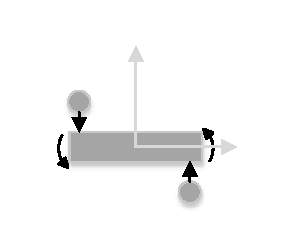
\includegraphics{avgProblem.pdf}
	\caption{Visualization of the averaging problem for point symmetric features. The circles represent the actuator while the rectangle represents a block object. Both pushing scenarios result in the same direction for orientation change of the object, however averaging the relative x and y positions would result in an invalid precondition.} 
	\label{fig:avgProblem}
\end{figure}

For point symmetric features, such as relative x and y positions in the figure, averaging results in invalid preconditions. In this case, the averaged preconditions would want the actuator to be in the center of the block, which is neither possible nor would it result in an orientation change. In order to prevent this, two averages are computed for each feature. One for all positive values of that feature and one for all negatives. on top of that, all combination of feature signs are stored and weighted by the magnitude of the change. When returning the entire preconditions, the averages corresponding to the sign combination with the highest weight are returned. Table \ref{tab:signCombinations} shows the combinations visible in the example above. In case combination 1 has the highest weight, the positive average for the x position, the negative average for the y position and the positive average for the y velocity is used. 

\begin{table}
	\centering
	\begin{tabular}{|c|c|c|}
		\hline Feature & Combination 1 & Combination 2 \\ 
		\hline x position & + & - \\ 
		\hline y position & - & + \\ 
		\hline y velocity & + & - \\ 
		\hline 
	\end{tabular} 
	\caption{Table showing the sign combinations for the example in figure \ref{fig:avgProblem}}
	\label{tab:signCombinations}
\end{table}

\subsection{Adapted instantaneous topological map \label{sec:ITM}}
%TODO Add pseudo code at the beginning to show general process or nice figure!
%TODO find better name! Consider calling it something closer to kNN since that is kind of what it becomes
The underlying regression and classification model that is used throughout this thesis is an adaptation of the \acrfull{itm} which will be called \acrfull{aitm} throughout this thesis.
The \gls{itm} \cite{itm} is an adaptation of the \gls{gng} \cite{gng} algorithm to create topological maps. Instead of \glspl{gng} global update rules for inserting new nodes in the map, the \gls{itm} uses local update rules in order to be better suited for correlated inputs. 
In order to be applicable to classification and regression, the \gls{itm} was further extended by an output function using the idea of \gls{llm} \cite{LLM}. In order to extend a topological map with an output function, each node represent the corresponding output vector $\vec{w}^i_{out}$ along its input vector $\vec{w}^i_{in}$. The \gls{llm} extends each node further with a local linear mapping $A^i$. This matrix is used to improve the function approximation within each Voronoi cell. With this, the output of each node given an input vector $\vec{x}$ is computed by equation \ref{eq:llmOut}:

\begin{equation}
\vec{y}^i(\vec{x}) = \vec{w}^i_{out} + A^i \cdot (\vec{x}-\vec{w}^i_{in})
\label{eq:llmOut}
\end{equation}

The output function for the net can be computed in multiple ways. The simplest method is to use the output of the winning node, i.e. the output of the node whose input vector $\vec{w}^i_{in}$ is closes to the given input $\vec{x}$. In order to reduce the effect of the metric problem when finding the closest node, the outputs of multiple nodes can also be mixed together. The evaluations in this thesis interpolate the output functions of the two closest nodes:

\begin{equation}
\vec{y}_{net}(\vec{x}) =  \frac{1}{k_n+k_s} \cdot \left[ k_n \cdot \left(\vec{w}^n_{out} + A^n \cdot \left(\vec{x}-\vec{w}^n_{in}\right)\right) + k_s \cdot  \left(\vec{w}^s_{out} + A^s \cdot \left(\vec{x}-\vec{w}^s_{in}\right)\right)\right]
\end{equation}

where $k_n$ and $k_s$ are the weights or importance for the nearest and the second node respectively. These weights are computed as follows:

\begin{equation}
\begin{split}
k_n = \exp\left(\frac{||\vec{x}-\vec{w}^n_{in}||}{\sigma^2}\right) \\
k_s = \exp\left(\frac{||\vec{x}-\vec{w}^s_{in}||}{\sigma^2}\right) 
\end{split}
\end{equation}

$\sigma$ determines the influence radius of each node, just like in radial basis networks \cite{rbf}. The nearest node $n$ and the second closest node $s$ are determined by comparing the input vectors of all nodes in $W$ with the given input vector $\vec{x}$:

\begin{equation}
\begin{split}
	nearest: n = \argmin_{c\in W} ||(\vec{x} - \vec{w}^c_{in})|| \\
	second: s = \argmin_{c\in W\backslash\{n\}} ||(\vec{x} - \vec{w}^c_{in})||
\end{split}
\label{eq:itmNearest}
\end{equation}

During training, the network receives an input-output pair and updates its nodes. First, the two closest nodes $nearest$ and $second$ are computed as stated in equation \ref{eq:itmNearest}. Afterwards, only the node $nearest$ is adapted:

\begin{equation}
\begin{split}
\Delta \vec{w}^n_{in} = \eta_{in} \cdot (\vec{x}^\alpha - \vec{w}^n_{in}) \\
\Delta \vec{w}^n_{out} = \eta_{out} \cdot (\vec{y}^\alpha - \vec{y}^n(\vec{x}^\alpha)) + A^n \cdot \delta \vec{w}^n_{in} \\
\Delta A^n = \eta_A \cdot (\vec{y}^\alpha - \vec{y}^n(\vec{x}^\alpha)) \frac{(\vec{x}^\alpha - \vec{w}^n_{in})^t}{||\vec{x}^\alpha - \vec{w}^n_{in}||^2}
\end{split}
\end{equation}

The initial matrix $A$ is a zero matrix with proper dimensions. The learning rates $\eta_{in}, \eta_{out}$ and $\eta_A$ are meta parameter that need to be determined. In case $\eta_A$ is set to 0, no linear approximation is learned for each Voronoi cell. This means, that each cell has only the constant output of $\vec{w}^n_{out}$.

After the winning node has been updated, the classical \gls{itm} algorithm uses local relations between the new input, the winning node and the second node in order to determine if a new node should be inserted or if some node should be deleted. As long as there are no big jumps in consecutive training samples, this approach works quite well. However, when resetting the environment between consecutive training runs, larger gabs can arise. Furthermore, this network has already been extended by an output function which can now also be used during training. This adapted \gls{itm} inserts new nodes into the network if the current network output varies too much from the target output, i.e if:

\begin{equation}
||\vec{y}^{net}(\vec{x}^\alpha)-\vec{y}^\alpha|| > \epsilon_{ITM}
\end{equation}

The threshold $\epsilon_{ITM} = 10^d$ is dynamically computed, based on the order of magnitude $d$ of the target output norm: %TODO example

\begin{equation}
d = \begin{cases}
\lfloor\log_{10}(||\vec{y}^\alpha||)\rfloor-1 & \text{if $||\vec{y}^\alpha|| > 0$} \\
-k & \text{otherwise}
\end{cases}
\end{equation}

When the output has a norm of $0$ a fixed threshold $10^k$ is chosen. Ideally $k$ should represent the average order of magnitude of the input. This average can be computed incrementally from the non-zero output norms. The benefit of such a dynamic threshold is that it automatically adapts to different use cases. For example, when the \gls{aitm} is used for classification, the output values will be class labels in the form of positive natural numbers. In this case $d=0$ which results in a threshold of 1. In regression tasks however, the output values will be real numbers. It is obvious that different thresholds are required for both types of use case. The \gls{aitm} assumes that the orders of magnitude of the output within one use case are generally rather similar and can be used as an approximation of the desired accuracy.

%TODO Subject to change
With every update the two winning nodes are connected as neighbors. Node deletions are performed just as in the traditional \gls{itm}: Second winners are removed if they are too far away from the winning node. Furthermore, isolated nodes will be deleted. A node is considered isolated if it does not have any neighbors left. Neighbor connections are removed if the second winner in an update can replace a previous neighbor:

\begin{equation}
\forall c \in N(n): \text{If~} (\vec{w}^n_{in}-\vec{w}^s_{in}) \cdot (\vec{w}^c_{in}-\vec{w}^s_{in}) < 0 \text{~remove connection (n,c)}
\end{equation}

$N$ denotes the set of neighbors of the winning node $n$.

%\subsection{Abstract inverse model}
%%TODO
%[TOOD maybe move description from concept here]
